\documentclass{article}
\usepackage[utf8]{inputenc}
\usepackage[spanish]{babel}
\usepackage{listings}
\usepackage{graphicx}
\graphicspath{ {images/} }
\usepackage{cite}

\begin{document}

\begin{titlepage}
    \begin{center}
        \vspace*{1cm}
            
        \Huge
        \textbf{Proyecto Parcial I}
            
        \vspace{0.5cm}
        \LARGE
        Informatica II
            
        \vspace{1.5cm}
            
        \textbf{Pedro Luis López Santiago}
        
        \textbf{Alejandro Lopera Gutierrez}
        
        \textbf{Juan David Jimenez Osorio}        
        
        \vfill
            
        \vspace{0.8cm}
            
        \Large
        Departamento de Ingeniería Electrónica y Telecomunicaciones\\
        Universidad de Antioquia\\
        Medellín\\
        Marzo de 2021
            
    \end{center}
\end{titlepage}

\tableofcontents
\newpage
\section{Introduccion}\label{intro}
Mediante el uso de herramientas nombradas y utilizadas en las clases de informatica II, de la Universidad de Antioquia, se llevara a cabo una serie de ejercicios y mecanismos utilizados para ejercer o darle forma a un proyecto, el cual será un panel de 8x8 leds, totalmente funcionable, el cual pueda reflejar cierta secuencia de iluminacion reflejando ante los ojos del receptor una forma conocida, ya sea un numero o una letra.
Se tendran en cuenta una serie de criterios y normas establecidas por el docente a cargo de la materia, como trabajar desde tinkercad, utilizando cierta cantidad de pines y tambien utilizando un integrado en especifico.
Tiene un alto nivel de logica el proyecto a trabajar y se necesitara de un desenvolvimiento en equipo donde todos los miembros de este trabajen de forma armonica para que puedan darle forma final con exito.

\section{Analisis del problema} \label{contenido}
Como problema a resolver, piden hacer un panel de leds 8x8 totalmente funcional, que refleje una secuencia especifica solicitada por el usuario.
Se debe trabajar bajo ciertos parametros establecidos.

-Trabajar con arduino 1

-No usar más de 7 pines

-Usar el integrado 74HC595

-Se debe incluir apuntadores y arreglos en el codigo utilizado

-Se necesita hacer un esquema

El proyecto se realiza en un equipo integrado por 3 estudiantes que analizaran, discutiran y trabajaran de manera armonica para completar la tarea con exito.
\section{Esquema Utilizado Para Formacion Del Codigo}
Pasos y procedimientos que se llevaron a cabo para la formacion del codigo



\subsection{código en el documento}
%
A continuación, se presenta el código \ref{codigo_ejemplo}, que nos permite incluir en el informe partes de programa que requieran una explicación adicional.
\begin{lstlisting}[language=C++, label=codigo_ejemplo]
// Programa desarrollado, compilado y ejecutado en https://www.onlinegdb.com
#include <iostream>

/*
 * Esto es un comentario de varias lineas
 */

// Comentario de una sola linea

#define N 10

using namespace std;

int main()
{
    
    for( int i = 0 ; i < N ; i++ ){
        
        if( !(i % 2) )
            cout << " El valor de i es -> " << i << endl;
    }
    
    return 0;
}

//Resultado programa

/*
El valor de i es -> 0
El valor de i es -> 2
El valor de i es -> 4
El valor de i es -> 6
El valor de i es -> 8
*/
\end{lstlisting}


\subsection{Problemas Al Realizar El codigo}
Aqui van los problemas que se tuvieron en la realizacion del codigo
\section{Conclusion} \label{Conclusion}
CONCLUSION DESPUES DE FINALIZADO EL PROYECTO
\section{Inclusión de imágenes} \label{images}
En la imagen (\ref{fig:circuito.PNG}), Se muestra el circuto ya completamente realizado.

\begin{figure}[h]
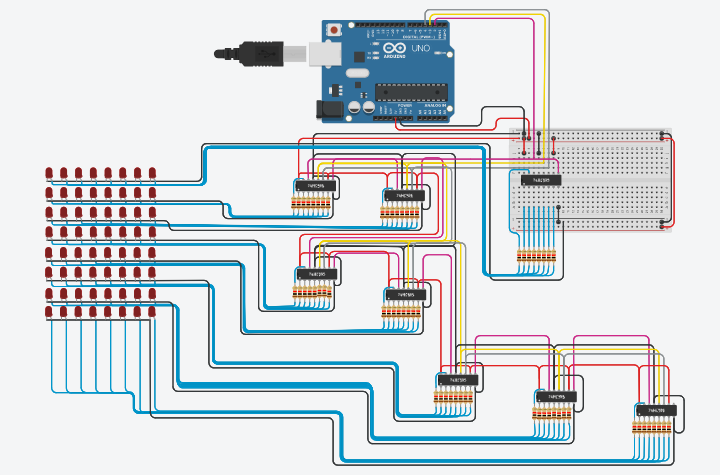
\includegraphics[scale=0.8]{circuito.PNG}
\graphicspath{ {images/} }
\centering
\caption{Circuito de los leds}
\label{fig:circuito.PNG}
\end{figure}

Las secciones (\ref{intro}), (\ref{contenido}) y (\ref{images}) dependen del estilo del documento.

\bibliographystyle{IEEEtran}


\end{document}
